
\chapter{Introduction}
\section{Purpose}
Data4Help is a service built to collect,organize and distribute the increasing amount of eHealth data generated by wearables.
\givespace
This service is built for two typologies of users:
\begin{itemize}
\item Third-Parties: users that want to access Data4Help collected data. These users will have access to the system by joining through a Web Application.
\item Individuals: users that want to provide their eHealth data to Data4Help. Data4Help will also collect additional individuals' information, in order to better organize and distribute the collected data.
These users will have access to the system by instead joining through a smartphone application.
\end{itemize}
Data4Help can be seen as the intermediary between eHealth data providers and eHealth data analyzers: it will gather  and store eHealth data from individuals and it will make the collected data accessible for any third party, respecting however individuals' privacy.
\givespace

The ability to gather eHealth data will be also used to build another service on top of Data4Help, called AutomatedSOS.
This service monitors the health status of a subscribed individual and when some vital parameters cross certain thresholds, sends to the user an ambulance.
\givespace

Improving individuals lifestyle and helping third parties to analyze their health status will be the key drivers of Data4Help features.
\givespace
Reading this document will be fundamental to better understand what is the role of Data4Help and what this service should provide to both its kind of users.





\section{Scope}
\subsection{Description of the given problem}
In a fragmented market, like the wearable one, Data4Help will act as a central hub for eHealth data.
Individuals will be able to use the supported wearables, in order to upload their data to the system through the smartphone application. In particular they will able to upload the following data from their wearable: steps taken, heart rate,sleep time and blood pressure.
\givespace
The collected data can be then accessed by third-parties in two different ways:
\begin{itemize}
\item Anonymized data: data of group of individuals, where the group is identified by giving constraints to the requested data. The constraints can be set on the individuals by specifying their age,sex or location or on the eHealth data by specifying intervals to each specific data. To maintain a certain level of privacy only requests that detect groups made of a number of individuals that is higher than 1000 are allowed by the system.
\item Specific individual data: specific individual data can be accessed only after the third-party had sent a data access permission request to the individual, and the request was accepted. The system will act as the intermediary, it will take the third party request and send it to the individual and will then notify the third party with the individual's response,giving access to his data if the request was accepted or by denying the access if the request was not accepted.
\end{itemize}
The system also gives the opportunity to third parties to be notified when new data is available, for both the specific individual data requests and the group requests.
\givespace
Individuals can also subscribe to another service, included in the application: AutomatedSOS. This service monitors the health status of an individual continuously, and, if certain parameters go below a critical threshold, the application starts automatically a rescue procedure. The rescue procedure should start in under 5 seconds from the crossing of the threshold and consists in sending an ambulance to the position of the user.
\givespace
To better understand what are the phenomena that are part of the system and what are not, consider the following diagram
\begin{figure}[H]
\centering
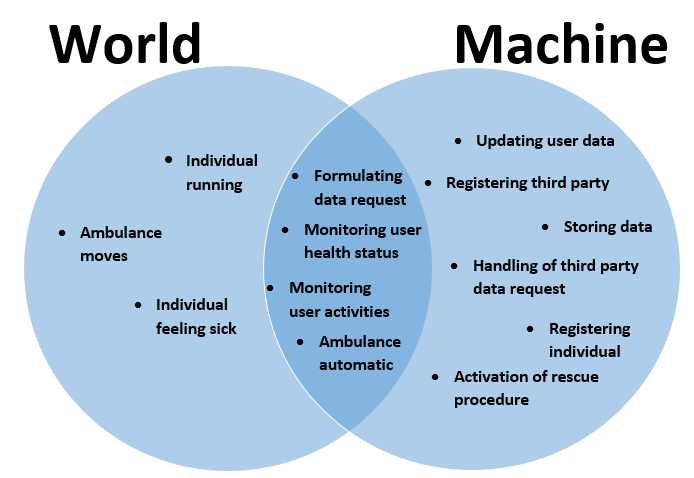
\includegraphics[scale=0.7]{resources/worldandmachine.png}
\end{figure}


\subsection{Goals}

\begin{itemize}
\item[] \goal{Individuals eHealth data is correctly gathered from their wearables.}{Data}
\item[]\goal{
Third parties can have access to accepted group data requests.
}{GroupData}
\item[]\goal{
Third parties can have access to data of specific individuals that gave permission to it.
}{SpecData}
\item[]\goal{
Third parties can receive updates whenever new data of their observed groups or individuals is gathered.
}{Notify}
\item[]\goal{
An ambulance is called whenever an individual vital parameter crosses a critical threshold.
}{Rescue}
\item[]\goal{
Users privacy cannot be violated.
}{Privacy}
\end{itemize}








\section{Definitions, acronyms, abbreviations}
\subsection{Definitions}
\begin{itemize}
\item \textbf{Rescue Procedure}: all the operations needed to save a person life. The operations include both the ones handled by computers and humans.
\item \textbf{eHealth Data}: all the data that can the related to the general health of the user, for example steps taken daily, hearth beat, blood pressure, activity level
\item \textbf{Health status}: level of health of a person, obtained analyzing various parameters like  hearthbeat rate, hours of sleep.
\item \textbf{Critical Treshold}: value that, referred to an health parameter, must not be passed to guarantee user vital activities.
\item \textbf{Wearable}: electronics that can be worn on the body, either as an accessory or as part of material used clothing. For the Data4Help system, only smartwaches will be initially considered.
\item \textbf{Data hub}: collection of data from multiple source organized for distribution.
\end{itemize}




\subsection{Acronyms}

\begin{itemize}
\item \textbf{TC}: Tax Code
\item \textbf{DBMS}: Database Management System
\item \textbf{DDoS}: Distributed Denial of Service
\item \textbf{GPS}: Global Positioning System
\end{itemize}

\subsection{Abbreviations}
\begin{itemize}
\item[Gn]: n-th goal
\item[Dn]: n-th domain assumption
\item[Rn]: n-th functional requirement
\end{itemize}



\section{Document Structure}
This RASD document is organized in the following way:
Chapter 1 contains an introductory overview on Data4Help, specifically it describes for which users this service is designed for and what are its main goals.
\givespace
Chapter 2 contains an overall description of Data4Help, starting from a class diagram that helps to visualize what is the model used to build this service and what is the role of Data4Help in it. A state chart diagram about the AutomatedSOS service is also included in order to better specify the main steps in order to guarantee this service. This chapter also provides a more specific description of Data4Help functionalities and its users, what are the constraints on these functionalities, and the domain assumptions
\givespace
Chapter 3 contains the following external interface requirements: user interface, hardware, software and communication interfaces. In particular the user interface section contains some mock ups that will serve as guideline to develop a suitable user interface for both the third parties and the individuals. 
This chapter also contains the functional requirements. The functionalities that are explicited through use case and sequence diagrams and with the help of some scenarios that describe concrete examples of Data4Help uses.
Non functional requirements are then defined, these requirements specify what are the performance and system properties needed to successfully guarantee the functionalities listed before.
\givespace
Chapter 4 contains the Alloy model used to validate some critical parts, parts that will be specified in an introductory description.
\givespace
Chapter 5 show how much time each group member has spent building this document.
\givespace
Chapter 6 includes the reference documents.